 \vskip 0pt plus -2fil
 \begin{IEEEbiography}
 [{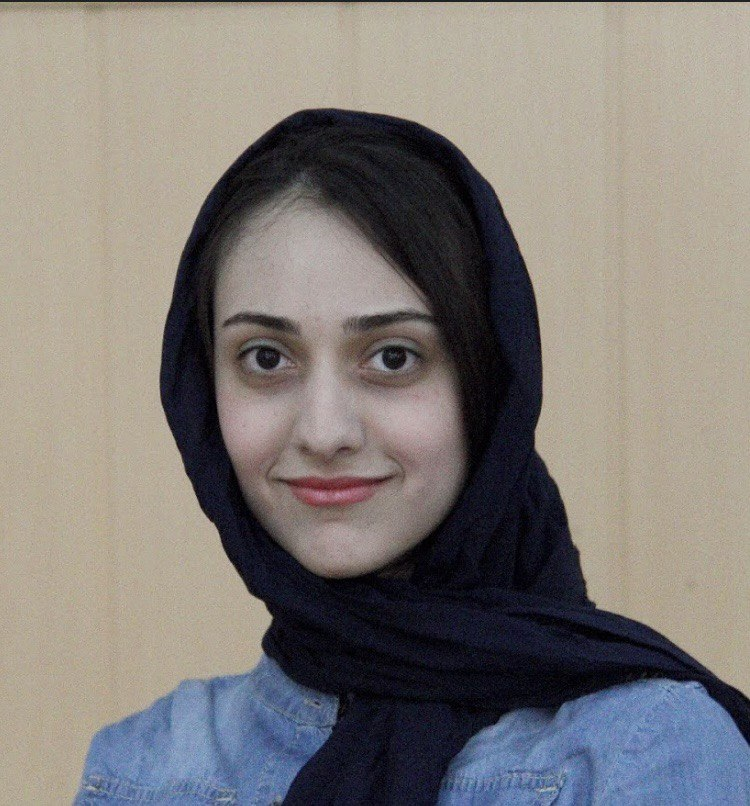
\includegraphics[width=1in,height=1.25in,clip,keepaspectratio]{bio/mojdeh.jpg}}]{ Mojdeh Karbalaee Motalleb (Karbalaeimotaleb)} received her B.S. and M.S. degrees in electrical engineering from the Amirkabir University of Technology, Tehran, Iran in 2015 and 2017. She is working toward a Ph.D. with the Department of Computer and Electrical Engineering, University of Tehran, Tehran, Iran. She is also a Visiting Research Student with the Center for Wireless Communications, Oulu University, Oulu, Finland. Her research interests include optimization and machine learning in network and wireless system.
 \end{IEEEbiography}
  \vskip 0pt plus -1fil
\begin{IEEEbiography}[{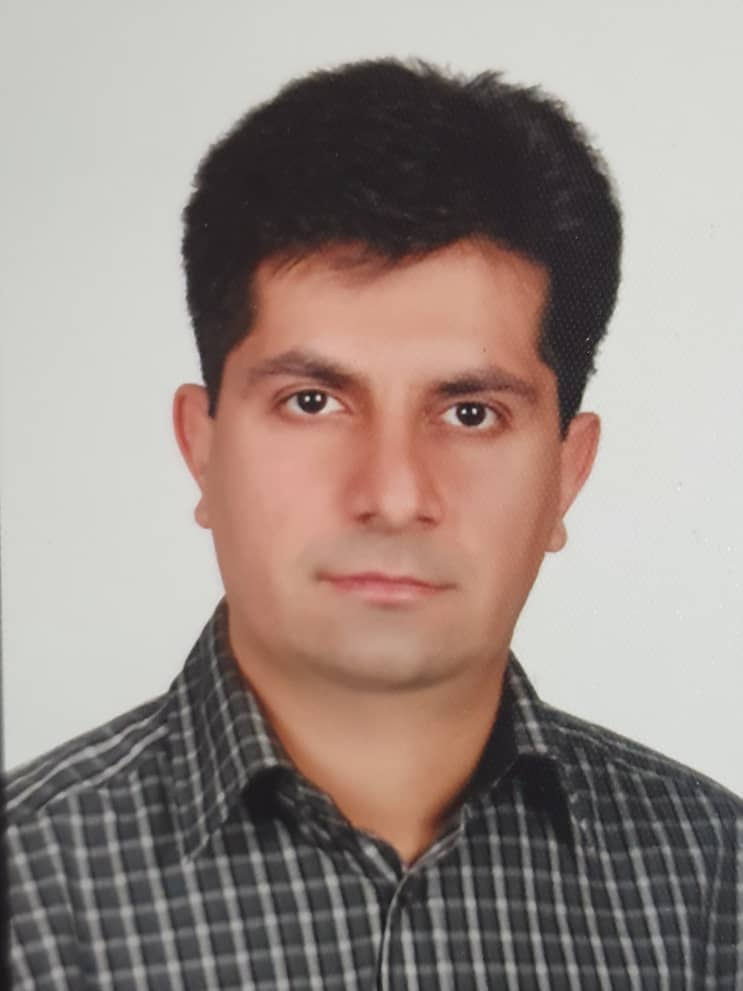
\includegraphics[width=1in,height=1.25in,clip,keepaspectratio]{bio/Vahid}}]{Vahid Shah-Mansouri}%%%IEEEbiographynophoto
(S’02–M’13) received the B.Sc. degree in electrical
engineering from the University of Tehran, Tehran, Iran, in 2003,
the M.Sc. degree in electrical engineering from Sharif University
of Technology, Tehran, Iran, in 2005, and the Ph.D. degree from The
University of British Columbia, Vancouver, BC, Canada, in 2011,
respectively. Since 2013, he has been with the
School of Electrical and Computer Engineering, University of Tehran,
Tehran, Iran. His research interests include analysis and mathematical
modeling of communication and computer networks.
\end{IEEEbiography}
 \vskip 0pt plus -1fil
\begin{IEEEbiography}[{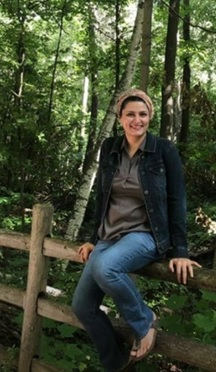
\includegraphics[width=1in,height=1.25in,clip,keepaspectratio]{bio/Saeedeh}}]{Saeideh Parsaei Fard}%%%IEEEbiographynophoto
 received the B.Sc. and M.Sc. degrees from the Amirkabir University of Technology (Tehran Polytechnic), Tehran, Iran, in 2003 and 2006, respectively, and the Ph.D. degree in electrical and computer engineering from Tarbiat Modares University, Tehran, in 2012. She is now part of Apple Cellular Platform Architecture team. Saeideh was a research scientist and lecturer from 2019 to 2021 at the University of Toronto, Canada. She was a Postdoctoral Research Fellow with the Telecommunication and Signal Processing Laboratory, Department of Electrical and Computer Engineering, McGill University, Canada, in 2013. From 2010 to 2011, she was a Visiting Ph.D. student with the Department of Electrical Engineering, the University of California at Los Angeles, Los Angeles, CA, USA. Her works are published in 3 books and 50 journals and conference papers, which are cited more than 1300 times with an h-index of 19 and i10-index of 31. She was awarded the “IEEE women in engineering award" in region 8 and Senior Member IEEE in 2018. Her background includes optimization theory, game theory, signal processing, and networking. Her current research focuses on distributed/federate learning, machine learning applications in next-generation wireless networks such as network automation and resource management, and robustness in both learning and communication. 
 \vspace{-1mm}
\end{IEEEbiography}
 \vskip 0pt plus -1fil
 \begin{IEEEbiography}
 [{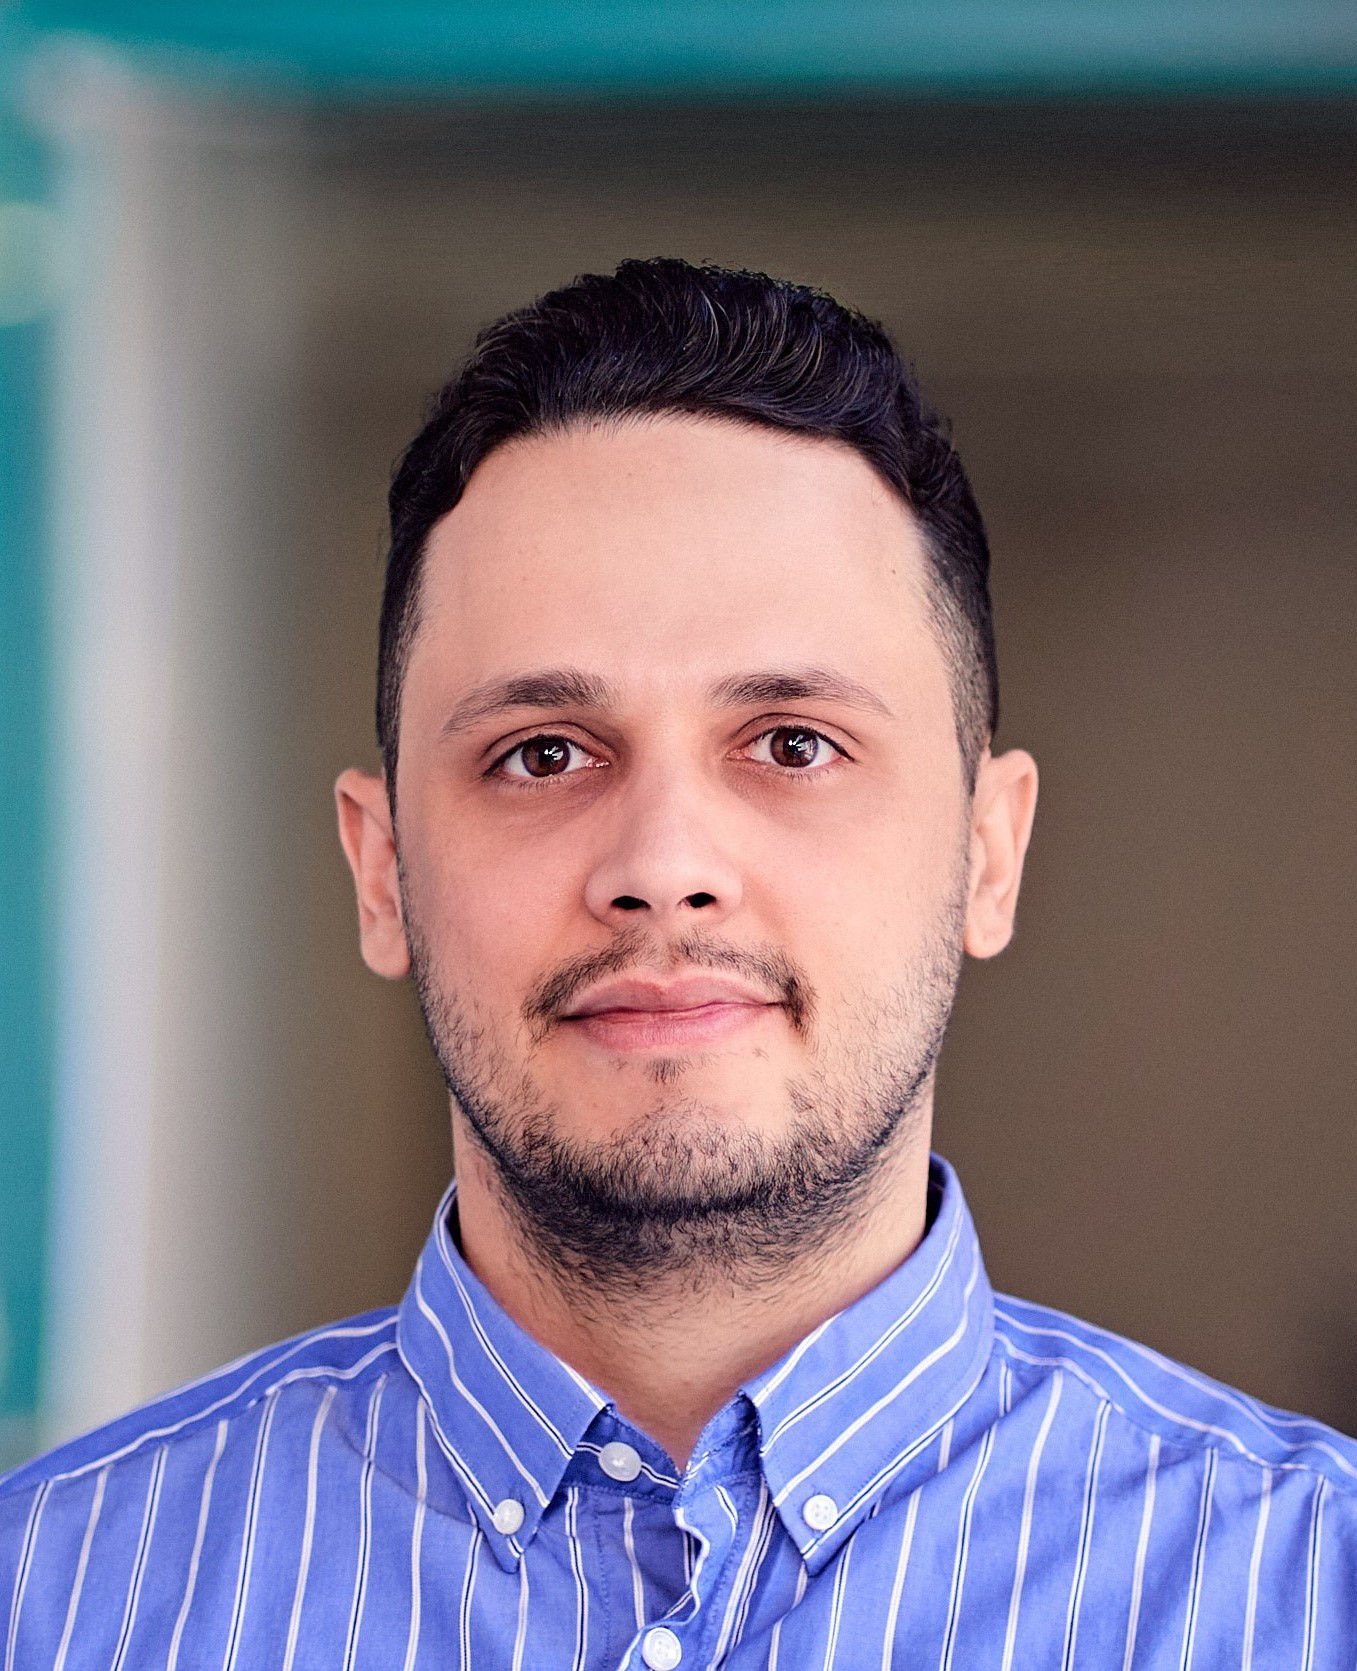
\includegraphics[width=1in,height=1.25in,clip,keepaspectratio]{bio/onel.jpg}}]{ Onel L. A. López} (S'17-M'20) received the B.Sc. (1st class honors, 2013), M.Sc. (2017) and D.Sc. (with distinction, 2020) degree in Electrical Engineering from the Central University of Las Villas (Cuba),  the Federal University of Paraná (Brazil), and the University of Oulu (Finland), respectively. From 2013-2015, he served as a specialist in telematics at the Cuban telecommunications company (ETECSA). He is a collaborator to the 2016 Research Award given by the Cuban Academy of Sciences, a co-recipient of the 2019 IEEE EuCNC Best Student Paper Award, the author of the best doctoral thesis in engineering in Finland in 2020, and the recipient of the 2022 Young Researcher Award in the field of technology in Finland. He is co-author of the book entitled ``Wireless RF Energy Transfer in the massive IoT era: towards sustainable zero-energy networks'', Wiley, Dec 2021. He currently holds an Assistant Professorship (tenure track) in sustainable wireless communications engineering in the Centre for Wireless Communications (CWC), Oulu, Finland. His research interests include sustainable IoT, energy harvesting, wireless RF energy transfer, wireless connectivity, and machine-type communications.
 \end{IEEEbiography}

